\documentclass[ejs]{imsart}
\usepackage[german,american,british]{babel}
%\usepackage[backend=biber,natbib=true,style=numeric,doi=true,url=true]{biblatex}
\usepackage{tgtermes}
\usepackage{caption}
\usepackage{subcaption}
\usepackage{multicol}
\usepackage{longtable}
\usepackage{booktabs}
\usepackage{array}
\usepackage{csquotes}
\usepackage{floatrow}
\usepackage{amsmath,amssymb,amsfonts}
\usepackage{listings}
\usepackage[hidelinks]{hyperref}
\usepackage{mathtools}
\usepackage{harpoon}
\usepackage{accents}
\usepackage{nicefrac}
\usepackage{wasysym}

\newcommand{\vect}[1]{\protect\accentset{\rightharpoonup}{#1}}
%\newcommand{\vect}{\protect\overset{\rightharpoonup}}
\DeclareMathOperator*{\argmin}{arg\,min}
\DeclareMathOperator*{\argmax}{arg\,max}

\RequirePackage{amsthm,amsmath}
\RequirePackage[numbers]{natbib}
\RequirePackage[colorlinks,citecolor=blue,urlcolor=blue]{hyperref}
\RequirePackage{graphicx}

% settings
\pubyear{2022}
\volume{0}
\issue{0}
\firstpage{1}
\lastpage{8}
\arxiv{2010.00000}

\startlocaldefs
\numberwithin{equation}{section}
\theoremstyle{plain}
\newtheorem{thm}{Theorem}[section]
\endlocaldefs

\begin{document}

\begin{frontmatter}
\title{The Optimally Weighted Median and its Variance}
\runtitle{The Optimally Weighted Median}

\begin{aug}
%\author{\fnms{Wolfgang} \snm{Brehm}\thanksref{t1,t2}\ead[label=e1]{wolfgang.brehm@desy.de}}
\author{\fnms{Wolfgang} \snm{Brehm}\thanksref{t2}\ead[label=e1]{wolfgang.brehm@gmail.com}}
%\address{Center for Free-Electron Laser Science CFEL, Deutsches Elektronen-Synchrotron DESY, Notkestr. 85, 22607 Hamburg, Germany \printead{e1}}
\address{Iserbrooker Weg 65, Hamburg \printead{e1}}

%\thankstext{t1}{I am thankful for the support from DESY (Hamburg, Germany), a member of the Helmholtz Association HGF.}
\thankstext{t2}{This publication is possible due to the support from the Cluster of Excellence ``CUI: Advanced Imaging of Matter'' of the Deutsche Forschungsgemeinschaft (DFG) -- EXC 2056 -- project ID 390715994.}
\runauthor{W. Brehm}
\end{aug}

\begin{abstract}
The weights that minimize the variance of the weighted median are proportional to the probability density of the samples at the overall weighted median.
If the weights are chosen optimally in this sense, the variance of the weighted median estimate will be inverse to four times the sum of probability densities at the weighted median.
\end{abstract}

\begin{keyword}[class=MSC]
\kwd[Primary ]{60K35}
\kwd{60K35}
\kwd[; secondary ]{60K35}
\end{keyword}

\begin{keyword}
\kwd{order statistics}
\kwd{weighted median}
\kwd{l1 optimization}
\end{keyword}
\tableofcontents
\end{frontmatter}

\section{Introduction}
The median is the most robust estimator of central tendency.
The weighted median is a straightforward generalization of the median, like the weighted mean is for the mean.
They can be generalized to higher dimensions, and computed in near linear time \cite{geometric_median_in_nearly_linear_time,centerpoint_in_linear_time}.

A different weighting of the samples, aside from the trivial frequency weighting, is preferred, when the samples are known to be not equally reliable.
Perhaps because they are on a different scale, measured differently, or not equally significant in some other way.
Sometimes unclear, however, is how to choose the weights for the weighted median exactly.
A similar problem arises in $L^1$ optimization with heterogeneous data points, because the median minimizes the $L^1$ norm.
For these cases, this publication will give some guidance.
To find the optimal weights, first, the variance of the equally weighted median will be recapitulated.
Secondly, the condition for optimality will be set and then the optimal weights will be derived, illustrated by numerical simulations.
And lastly, results and implications will be discussed.

The median value of a distribution is the value where the cumulative distribution equals $\nicefrac{1}{2}$, meaning values less than or equal the median are just as likely as values larger than or equal \cite[Chap.~2.8]{kendall1945}.
Just like the mean of a distribution can be estimated with the sample average, the median of a distribution can be estimated with the sample median.
When there is an even number of samples, all values between and including the two middle most values are median values according to the definition.
And like there is the central limit theorem for the median, there is the median theorem for the sample median:

The median $\tilde{\mu}_s$ of a sample of size $N$ drawn from a distribution with density $p(x)$ approaches a Gaussian distribution with mean $\tilde{\mu}$ and variance $\left(4 N \left(p\left(\tilde{\mu}\right)\right)^2\right)^{-1}$ for large sample sizes, if the density around the median of the distribution is continuously differentiable and non-zero \cite[Supp.~mat.]{MILLER2017} \cite{doi:10.1080/01621459.1960.10482056}.
\begin{align}
\sigma^2_{\tilde{\mu}_s} = \dfrac{1}{4 N \left(p\left(\tilde{\mu}\right)\right)^2} \label{median_density_variance}
\end{align}
%\clearpage
To estimate the standard deviation of the sample median of samples from an unknown distribution, Woodruff\cite{Woodruff1952} suggests using the following formula:
\begin{align}
\sigma_{\tilde{\mu}_s} \approx \dfrac{ x_{\lceil \frac{1}{2}\left(N+\sqrt{N}\right) \rceil} - x_{\lfloor \frac{1}{2}\left(N-\sqrt{N}\right) \rfloor} }{2} \label{standard_deviation_median}
\end{align}
Because the median, by definition, is the value for which half the values are less than or equal and the other half is greater than or equal, the probability of a value at position $i$ in a ordered list of random samples being closest to the true median follows a binomial distribution with a success probability $p$ of $\nicefrac{1}{2}$.
Therefore the values at these positions correspond to $\tilde{\mu}+\sigma_{\tilde{\mu}}$ and $\tilde{\mu}-\sigma_{\tilde{\mu}}$ on average respectively, and their difference, on average, is about two times the standard deviation.
Knowing that the probabilities follow a binomial distribution, one can calculate a weighted squared deviation of the random samples to the sample median (analogous to the sample variance of the mean), to improve the accuracy of the variance estimate slightly at the cost of robustness:
\begin{align}
\sigma^2_{\tilde{\mu}_s} \approx \sum_{i=0}^{N-1} {N-1 \choose i} \left(\frac{1}{2}\right)^{1-N} \left(x_i - \tilde{\mu}_s\right)^2 \label{variance_median}
\end{align}

Because the median of a large random sample approaches a Gaussian distribution, it is sensible to try to minimize its variance for the most accurate estimate.
The optimal weights are the ones that minimize the variance of the weighted median.

\section{Derivation of the optimal weighting and the resulting variance}

We assume all samples $x_i$ can follow a different probability distribution $p_i\left(x\right)$, otherwise different weighting would have only very limited application and the non-weighted median would almost always be the preferred choice.
Consider a sorted list of weighted samples and the running sum of weights normalized by the sum of all weights.
This computes the empirical cumulative distribution of the weighted mixture distribution, let the weighted cumulative distribution be ${_wP}\left(x\right)$.
\begin{align*}
{_wP}\left(x\right) = \dfrac{\left( \sum_i^N w_i \int_{-\infty}^x p_i\left(y\right) dy \right)}{\left( \sum_i^N  w_i \right)}
\end{align*}

\noindent Now consider the sum of weights associated with samples less than or equal to the true weighted median ${_w\tilde{\mu}}$, normalized by the sum of all weights, let it be $c$:
\begin{align}
c = \dfrac{\left( \sum_{ \left\{ i | x_i \le {_w\tilde{\mu}} \right\} } w_i \right)}{\left( \sum_i^N  w_i \right)} \label{equation_c}
\end{align}
%\clearpage
\noindent Without knowing the median of each distribution, each weight has probability $\nicefrac{1}{2}$ of being part of this sum or its counterpart.
The variance introduced to the nominator by each weight is therefore $\nicefrac{1}{4}$ the weights squared and the variance of $c$ is approximated by the sum of individual variances divided by the normalization factor squared:
\begin{align*}
\sigma^2_c = \dfrac{\left(\sum_i^N w_i^2\right)}{4 \left( \sum_i^N  w_i \right)^2}
\end{align*}

\begin{figure}[b!]
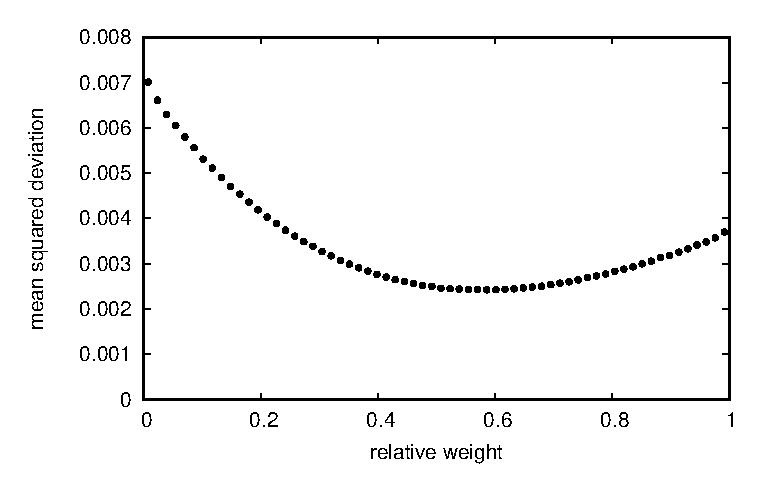
\includegraphics[width=10cm]{optimal_weighting_median.eps}
\caption{Relative weighting between samples following a Gaussian or uniform distribution with identical variance each. The ratio of the Gaussian density to the uniform density at the median is $\sqrt{\nicefrac{6}{\pi}} \approx 1.38$ , this ratio is reached at around $0.58$ on the x-axis, coinciding with the minimum of mean squared deviations of the weighted sample median to the actual median.}\label{median_weights}
\end{figure}

\noindent The weighted sample median ${_w\tilde{\mu}_s}$ is the sample where the empirical weighted cumulative distribution reaches $\nicefrac{1}{2}$.
The expected value of $c$ is $\nicefrac{1}{2}$ and its variance is the mean squared deviation between the empirical partitioning which determines the weighted sample median and the partitioning which would lead to the value closest to the weighted population median.
Therefore the value where the weighted cumulative distribution reaches $c$ has the same variance as the weighted median.
Error propagation demands the derivative of ${_wP^{-1}}$ at $\nicefrac{1}{2}$ which is inverse to the derivative of ${_wP}$ at the weighted population median.

\begin{align*}
\sigma^2_{_w\tilde{\mu}_s} &= \sigma^2_c \dfrac{d{_wP^{-1}}}{dx} \left(c\right)\\
\sigma^2_{_w\tilde{\mu}_s} &= \sigma^2_c \left(\dfrac{d{_wP}}{dx} \left({_w\tilde{\mu}}\right)\right)^{-1}\\
\sigma^2_{_w\tilde{\mu}_s} &= \dfrac{\left(\sum_i^N w_i^2\right)}{4 \left( \sum_i^N  w_i \right)^2} \dfrac{\left( \sum_i^N  w_i \right)^2}{\left( \sum_i^N  w_i p_i\left({_w\tilde{\mu}}\right)\right)^2} \\
\sigma^2_{_w\tilde{\mu}_s} &= \dfrac{\left(\sum_i^N w_i^2\right)}{4 \left( \sum_i^N  w_i p_i\left({_w\tilde{\mu}}\right)\right)^2}
\end{align*}

\noindent This is the variance we seek to minimize and a very similar optimization problem to the optimal weights for the weighted average.
The weights that minimize the variance of the weighted median are reciprocal to the probability density of the sample distribution at the median, as can be shown by taking the first and second derivatives with respect to the individual weights.
The first derivative can only be zero for $w_i = p_i\left({_w\tilde{\mu}}\right)$ and the second derivative is positive, which are the necessary and sufficient conditions for a global minimum:
\begin{align*}
\dfrac{d \sigma^2_{_w\tilde{\mu}_s}}{d w_j} &= \dfrac{ w_j \left( \sum_i^N  w_i p_i\left({_w\tilde{\mu}}\right)\right) - p_j\left({_w\tilde{\mu}}\right) \left(\sum_i^N w_i^2\right)}{2 \left( \sum_i^N  w_i p_i\left({_w\tilde{\mu}}\right)\right)^3} \\%x/(2*(p*x+b)^2)-(p*(x^2+a))/(2*(p*x+b)^3)
\dfrac{d^2 \sigma^2_{_w\tilde{\mu}_s}}{d^2 w_j} &= \dfrac{1}{2 \left( \sum_i^N  w_i p_i\left({_w\tilde{\mu}}\right)\right)^2} - \dfrac{2 w_j p_j\left({_w\tilde{\mu}}\right)}{2 \left( \sum_i^N  w_i p_i\left({_w\tilde{\mu}}\right)\right)^3} + \dfrac{3 \left( p_j\left({_w\tilde{\mu}}\right)\right)^2 \left(\sum_i^N w_i^2\right)}{2 \left( \sum_i^N  w_i p_i\left({_w\tilde{\mu}}\right)\right)^4} %1/(2*(p*x+b)^2)-(2*p*x)/(p*x+b)^3+(3*p^2*(x^2+a))/(2*(p*x+b)^4)
\end{align*}
\begin{align}
\argmin_{w_i} \sigma^2_{_w\tilde{\mu}_s} = p_i\left({_w\tilde{\mu}}\right) \label{optimal_median_weights}
\end{align}

\noindent Numerical experiments as shown in figure~\ref{median_weights} also confirm this result.
When the weights are set proportional to $p_i({_w\tilde{\mu}})$, the variance of the median is equal to $\nicefrac{1}{4}$ the inverse of the sum of probability densities at the median squared: %(compare figure~\ref{weighted_median_variance}):
\begin{align}
\sigma^2_{_w\tilde{\mu}_s} &= \dfrac{1}{4 \left(\sum \left(p_i\left({_w\tilde{\mu}}\right)\right)^2\right)} \label{variance_of_weighted_median}
\end{align}

%\begin{figure}[b!]
%\includegraphics[width=9cm]{weighted_median_variance_estimate.eps}
%\caption{Numerical experiment with inverse density weighted Gaussian random samples of different size. The mean squared deviation of the weighted median is described well by equation~\ref{variance_of_weighted_median} as a function of the sum of squared weights, which is indicated by the red line.} \label{weighted_median_variance}
%\end{figure}

When the weights are proportional, they are still optimal, but estimating the variance from the weights directly with equation~\ref{variance_of_weighted_median} is not possble any more because the proportionality constant is unknown.
The variance can still be estimated analogous to equations~\ref{standard_deviation_median} and~\ref{variance_median}.
\begin{align}
\sigma^2_{_w\tilde{\mu}_s} &\approx \sum_i^N \left(x_i - {_w\tilde{\mu}_s} \right)^2 \int_{\sum_j^{i-1} w_i}^{\sum_j^i w_i} \exp \left(-\dfrac{1}{2} \left( \left(y-\dfrac{1}{2}\right)^2 \sigma_c^{-2} + \log \left(2 \pi \sigma_c^2 \right) \right) \right) dy \label{weighted_median_variance_estimate}
\end{align}
%The distribution of $c$ (equation \ref{equation_c}) approaches a Gaussian distribution with variance $\sigma_c^2$ for many samples, an exact solution is not known.

\begin{figure}[t!]
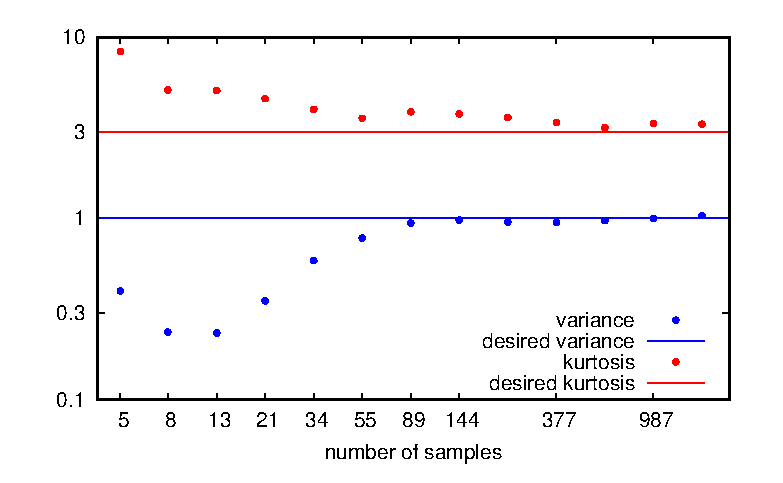
\includegraphics[width=10cm]{weighted_median_variance_kurtosis.eps}
\caption{Variance and kurtosis of the weighted sample median divided by its estimated standard deviation (equation \ref{weighted_median_variance_estimate}). The samples are drawn from a scaled normal distribution, where the weights are drawn from an exponential distribution and the divisors are set accordingly.} \label{median_variance_kurtosis}
\end{figure}

%\begin{figure}[b!]
%\includegraphics[width=9cm]{variance_exponent_median.eps}
%\caption{The median of absolute deviations of the sample median of samples following either a Gaussian, a Laplacian or a uniform distribution, with variances following an exponential distribution. The weights are set to a power of the associated sample variances and as can be seen the optimal exponent is around $-\nicefrac{1}{2}$.} \label{median_weights2}
%\end{figure}

\section{Discussion}

%One possibly unexpected consequence of weights proportional to the probability density at the median is that when the distribution of each sample has the same location and shape, and only differs in scaling, the optimal weights are proportional to the inverse standard deviation as demonstrated in figure~\ref{median_weights2}, not inverse variances as for the weighted average.


One possibly unexpected consequence of weights proportional to the probability density at the median is that when the distribution of each sample has the same location and shape, and only differs in scaling, the optimal weights are proportional to the inverse standard deviation, not inverse variances as for the weighted average.
This is because a scaling by a factor amounts to a linear decrease of the density at the median, but an increase of the variance by the same factor squared.

As can be seen in figure~\ref{median_variance_kurtosis} the distribution of the weighted sample median approaches a normal distribution asymptotically, but not immediately.
With fewer samples, the distribution can have significant excess kurtosis, typically being leptokurtic with a kurtosis above three, hinting to heavy tails, and making accurate estimation of a standard deviation difficult or possibly pointless.
The average or median of absolute deviations could be a better measure of precision in these cases.
\bibliographystyle{imsart-number} % Style BST file (imsart-number.bst or imsart-nameyear.bst)
\bibliography{ref}

\end{document}
